\documentclass{sig-alternate-05-2015}
\usepackage{listings}
\usepackage{wrapfig}

\begin{document}


\title{Avalanche Simulation in a Particle System}
\subtitle{As a part of the Master - Module 3D-Animation in the Hochschule Rhein Main
purely written in Python and OpenGL}
%
% You need the command \numberofauthors to handle the 'placement
% and alignment' of the authors beneath the title.
%
% For aesthetic reasons, we recommend 'three authors at a time'
% i.e. three 'name/affiliation blocks' be placed beneath the title.
%
% NOTE: You are NOT restricted in how many 'rows' of
% "name/affiliations" may appear. We just ask that you restrict
% the number of 'columns' to three.
%
% Because of the available 'opening page real-estate'
% we ask you to refrain from putting more than six authors
% (two rows with three columns) beneath the article title.
% More than six makes the first-page appear very cluttered indeed.
%
% Use the \alignauthor commands to handle the names
% and affiliations for an 'aesthetic maximum' of six authors.
% Add names, affiliations, addresses for
% the seventh etc. author(s) as the argument for the
% \additionalauthors command.
% These 'additional authors' will be output/set for you
% without further effort on your part as the last section in
% the body of your article BEFORE References or any Appendices.

\numberofauthors{2}
\author{
%
% The command \alignauthor (no curly braces needed) should
% precede each author name, affiliation/snail-mail address and
% e-mail address. Additionally, tag each line of
% affiliation/address with \affaddr, and tag the
% e-mail address with \email.
%
% 1st. author
\alignauthor
Tiras Zemicael\\
       \affaddr{Karl-Blum-Allee 57, 65929 Frankfurt am Main}\\
       \email{Tiras.Zemicael@student.hs-rm.de}
% 2nd. author
\alignauthor
Simon Rininsland\\
       \affaddr{Roseggerstrasse 5, 65187 Wiesbaden}\\
       \email{Simon.Rininsland@student.hs-rm.de}
}


\maketitle
\begin{abstract}
@Tiras Erklärung weg und sachen ergänzen. 
(What did we do. As tiny as possible)\\
- the question(s) you investigated (or purpose), (from Introduction)\\
	- state the purpose very clearly in the first or second sentence.\\
- the experimental design and methods used, (from Methods)\\
	- clearly express the basic design of the study.\\
	- Name or briefly describe the basic methodology used without going into excessive detail-be sure to indicate the key techniques used.\\
- the major findings including key quantitative results, or trends (from Results)\\
	- report those results which answer the questions you were asking\\
	- identify trends, relative change or differences, etc.\\
- a brief summary of your interpetations and conclusions. (from Discussion)\\
	- clearly state the implications of the answers your results gave you.\\
\\
\\
An Avalanche. A natural dreaded force of many snow and ice particles rushing down a Slope, driven by the Gravity. As many as snowflakes and ice particles which are included in an avalanche as good as we can play with them in an Particle System. One of the best examples for dynamicly rendered simulations for Particle Systems a snow Avalanche will be the central Part in our Project.\\
In order also to start just from the basics we decided to not use huge frameworks and start from the OpenGL Scatch. We will just use OpenGL Basics.\\ 
\\

We will solve some Physically based Problems which comes around with the Topic of an Avalanche like:\\
- Particles with seperated masses, driven by a force.\\
- Physically Effects, bouncing Particles and combining ones.\\
and some OpenGL based Problems like: \\
- shadow for every seperated Particle \\
- performance Issues and optimization.\\ 

We have developed a piece of Software, we want to simulate a physic driven avalanche. The Core features are mainly dedicated to understand and solving physical Problems. We created Particles which reacts on physical forces from outside. These happens physically correct. After that we took some work to give the Particles a good-looking view, which should give a better understanding what we try to simulate at the first look. \\

\end{abstract}


\begin{CCSXML}
<ccs2012>
<concept>
<concept_id>10010147.10010371.10010352.10010379</concept_id>
<concept_desc>Computing methodologies~Physical simulation</concept_desc>
<concept_significance>300</concept_significance>
</concept>
</ccs2012>
\end{CCSXML}

\ccsdesc[300]{Computing methodologies~Physical simulation}




\section{Introduction}
In the current time Simulation for almost everything exist. Simulations are a important part of todays society and is used for everything that can’t be test on a large scale or can’t even be create. The simulations are created to see possible situation or behavior of different thinks, for that the simulations need to be precise. Simulations are for the most parts not only a programming problem but also a problem in the subject the simulations are aiming for. Simulations need to behave the exact same as the real world counterpart, therefore a lot of physics is involved in such a simulation. And one of the highest requested kind of simulations are for weather phenomena. For that kind of problem simulations for every kind of weather phenomena exist. There are simulations for tidal waves, thunderstorms, flood and for our project Avalanche.
\subsection{Project Description}
The Project for our student module 3D-Animation was to make an avalanche simulation with the help of whatever graphic tool we want. We decided to use Python as our Programming language and the Python binding package for OpenGL. This two tools where the only greater tools that we used for the Project and for the Physics engine we decided to make it on our own so we could be self-sufficient and have the background knowledge behind the commonly used physics engine. With this as our tools we try to make a particle system for creating snow and behave the physically correct way for snow.
\subsection{Project Result}
The Result of the Project is a functional Simulation of an Avalanche. The finished code gives the possibility to change the snow amount and the objects for the snow and texture, it is also possible to change the mode for the simulator to debug to see the grid system and the corresponding collision information. 
\section{Technology}
\subsection{Python}
The Programming Language that is going to be used in this Project is Python. The version that we are going to use is the 2.7 Version and we are going to use it for the compatibility that this version has with the OpenGL python binder. Python is an easy to learn script base language that has a lot of possibility to use it. Python has a huge Community that contribute to the development of different packages and with the easy installer the usability is quite easy. The Python package manager pip helps us with the installation for the OpenGL binder pyOpenGL.
\subsection{OpenGL}
OpenGL is a cross-language and cross-platform graphics library which allows us to draw in our application. OpenGL helps us to draw and manipulate geometric figures and create scenes with a camera and light in a 3d environment. OpenGL exist since 1992 and it is mainly used for computer-aided design, virtual reality application, visualization of information and scientific results and in the videogames branch.
\subsection{Other Packages}
\section{Architecture}
Our Program inherits different Classes. The main Architecture can be described as follows:\\
All Objects in the World are described in the Objects class. Now, we have a Terrain and many particles. Both are implemented through the Object Class. A Particle inherits from the Objects Class, but uses some of the functions from the Objects Class. The World Class holds the Modell of our Program. \\
To have a Modell in our Program we need places to hold our Data. We took Numpy to store the position of every Particle in a global Grid-System.\\
Our Architecture must inherit a place to store all Particle Positions and must depict the Terrain. Because we saw fast, we can implement the Terrain Storage in a 2-dimensional Terrain, we decided to use two Arrays to store our Data. \\
\subsection{Main Class}
In every Program a Main Class is used to setup and initialised the Program. In our case, we use it to include all used external sources like OpenGL or our external OBJ-Loader, setting up the Scene, enable Options in OpenGL, registering mouse and keyboard functions and build the Window. In every loop Step from OpenGL we call the Objects Class draw function to enforce the calculation and displaying for the new Frame.\\
\subsubsection{Parameters}
In the Main Class, we can set some Parameters to influence the output of the Simulation. All Parameters are placed in the Header. Important Parameters are:\\
- emitterCount(Integer): Sets the number of emitter Flakes. Only EmitterFlakes gets fully physically correct calculated. \\
- flakesPerEmitter(Integer): Sets the number of Flakes for each Emitter Particle. In Order to get 3 Flakes visible, you can set emitterCount to 3 or set emitterCount to 1 and add 2 flakesPerEmitter. Performance will be better if having more FlakesPerEmitter as emitterCount, but it’s less realistic.\\
- Debug(boolen): Enables or disables the debug mode. More to debug Mode described later. \\
- Fps(Integer): Sets the maximum Frames per Second.\\
\subsubsection{Options setting in Code}
- To set the Camera starting Point you can change the "gluLookAt" function.\\
- To change the Flakes spawning Position range, you can change the lines 329-330:\\
\begin{lstlisting} [language=Python]
drawObjectsArray.append(particle.particle(
[uniform(-5.0, 5.0), uniform(50.0, 60.0), 
uniform(0.0, 55.0)],[0.0, 0.0, 0.0],
 uniform(.2, 1.0), 'resources/flake.obj',
 i, world, drawObjectsArray,
 flakesPerEmitter))
\end{lstlisting}
Change the 3 uniform values to set a random X, Y and Z range. \\
\subsubsection{Debug Mode}
We recognized fast, we need a debug Mode to have a better View of all our Calculations. To enable the Debug Mode, simply change the Debug Parameter described in the top to true. \\
In the Debug mode code, you can disable and enable single Viewable outputs of the Program. Things you can enable:\\
-	Position of the Flake in green: To see a bigger, more visible Flake you can set the first debug Mode to true. It enables a green box around each Flake.\\
-	Flake Vortex. To see the Vortex a single Flake is registered, you can enable the second debug Mode.\\
-	Flakes Collision Face: Each Flake creates an own Collision Face in each Frame. To see this, enable the third debug Option. \\
-	TerrainMap Points: To see the Terrain heightmap array on the Terrain, enable the fourth Option.\\
-	The last two Debug Options are dedicated to the World Grid. It enables a view of the World Grid. Caution: The Program is getting really slow and not usable if enabling this Options.\\

\subsection{Object Class}
The Object class holds many of the information dedicated to an object in our View. At the moment, we have two kinds of objects. The Terrain and our Particles. Bot need some properties and functions which are coded in the Object Class. \\
Some common Functions:\\
\subsubsection{The Draw Function}
The Object Class holds the draw function, which is the entry point for each loop Call from the Main Class. The draw function uses the draw function from the external OBJ Loader and does the translation for the position at each frame. Furthermore, it checks if the given Object is an Object (the Terrain) or a Particle. To only calculate the new position for the Particles and not for the Terrain.  \\
\subsubsection{The getHeightmap Function}
To calculate the heightmap for the Terrain, which is stored in the World Class, we need to calculi it somewhere. We wrote a function to loop through all the faces in the obj file and map the y value of it on the x and z Index of the 2-dimensional Array with:\\
\begin{lstlisting} [language=Python]
x = int(round(vertice[0])) 
+ world.worldSize
y = vertice[1]
z = int(round(vertice[2])) 
+ world.worldSize

world.terrainHeightMap[x][z] = y

\end{lstlisting}
Because of rounding errors in the height, we had some false Zeros in our Array which gets fixed afterwards with calculating the middle sum of the both neighbours from a face.\\
\subsubsection{The getBound Function}
To get the bound of our objects we need to get the vertex of the object. To get this we had to make a few adjustments on the obj-loader so it can support us with our procedure. The modified obj-loader can save the vertex in a separate list that can be used for the bounding functionality, with the list for all dimension we can now get the boundings, for this we need the highest and lowest entry for each dimension. With our values we can now create a bounding box with the following points.
\begin{table}[!htbp]
\centering
\begin{tabular}{llll}
        & Dim-X & Dim-Y & Dim-Z \\
Point 1 & min   & min   & min   \\
Point 2 & max   & min   & min   \\
Point 3 & min   & max   & min   \\
Point 4 & max   & max   & min   \\
Point 5 & min   & min   & max   \\
Point 6 & max   & min   & max   \\
Point 7 & min   & max   & max   \\
Point 8 & max   & max   & max  
\end{tabular}
\caption{bounding box points}
\label{my-label}
\end{table}
This are our corner points for the bounding box which we are going use for the collision detection and other things.
\subsubsection{The collisionDetection and collisionResponse Functions}
These 2 functions are only abstract methods to get implemented by the particle Class.\\
\subsection{Particle Class}
The Particle Class inherits from the Object Class and can use all the properties and functions from the Object Class.
\subsubsection{Header Parameters}
The first Thing visible if firstly checking this class are the two Parameters at the Top. Gravitation and collisionDistanceThreshold are nearly self explainable. In our Case the Gravitation is a vector with 3 Parameters. \\
\begin{lstlisting} [language=Python]
gravitation = [0, -9.81, 0]
\end{lstlisting}
The gravitation on the X and Z Axis is zero we all know. But the Gravitation on Y Axe is negative. Because the Gravitation is pulling all Objects to the bottom and not forcing them to the top. \\
The collisionDistanceThreshold described the threshold of the Moment a collision with the Terrain is really a collision. It never collides exactly with the Terrain, because the Movement is calculated once per Frame. It’s always a bit over or under the Terrain. This Parameter can be set lower or higher to gain more accuracy or have less Flakes fallen through the ground.\\

\subsubsection{A Particle}
A Particle has some characteristics in our Simulation. Some are equal to the Terrain like the position, or the obj where all the vertices are stored, but most of the Properties are only set on the Particle:\\
-	an index, to write it in the Vortex in world\\
-	Speed to gain or lose and have a flowing movement\\
-	Elasticity to set the force, which will be reflected from a collision\\
-	A Mass to set the weight and size of the flake\\
-	An Air Drag to lose speed, while drizzle to the terrain\\
-	A Voxel to store the Vortex in the World Grid\\
-	A collision Face to use later for collision and \\
-	The number of Spawned Flakes for each flake which gets calculated\\
\\
To later calculate the collision, we push some parameters through the simulation like drawObjectsArray, where all Objects in our World gets stored. To apply some randomness for the emitter Flakes we directly calculate some random position for each spawn Flake. \\

\subsubsection{Steps in every Frame}
In each Frame the next position of a Flake gets recalculated. The steps for a new position starts with the calculation if there could be a collision with the Terrain or another Particle. This is described later. \\
If there is no Collision we need to calculate the new Speed with:\\
\begin{lstlisting} [language=Python]
self.speed[0] += gravitation[0] * 
(1 - self.airDrag) * (dt / self.mass)
self.speed[1] += gravitation[1] * 
(1 - self.airDrag) * (dt / self.mass)
self.speed[2] += gravitation[2] * 
(1 - self.airDrag) * (dt / self.mass)
\end{lstlisting}
We see, that the new speed is the old speed add by some multiplied factors which have direct influence on the Flakes Seed like the Gravity, the air Drag and the mass of the Flake. To now get the new position it’s enough to simply say: \\
\begin{lstlisting} [language=Python]
self.position[0] += self.speed[0] * passed
self.position[1] += self.speed[1] * passed
self.position[2] += self.speed[2] * passed
\end{lstlisting}
Now we have the new position of our Flake. In the next Step, we give a look at the new position and check if we changed our voxel. If we left our old Voxel we must deregister the index of the Flake in the old one and register in a new one. If in the new one is no other index of a particle we simply register in the new one, if there is already one we have to check for a collision with another Flake in the one and write both or more in the new Voxel. \\
After that we draw our Flake in the world, which is separated in the world Class. \\


\subsection{World Class}
Our World Class stores the main Data in our Program. We have used a direct mapping from the real view World to our Modell. The Terrain has a 128 Unit Width and Length. On the top, we need 2 Units to have an invisible Wall. Regarding these two Unit Rules, we need to have a 130 Units big 3-dimensional Array. Because Numpy is very fast in creating those huge arrays, we used Numpy to create the Array. \\
With:\\
\begin{lstlisting} [language=Python]
self.grid = np.zeros((self.gridResolution, 
self.gridResolution, self.gridResolution),
 dtype=int)
\end{lstlisting}
We create fast a needed Array filled with zeros in Integer Type. We use Integer Types because we only need Integer values in our Array. Why is described later. Because we used -1 to set a Grid as not used, we must fill the array with:\\
\begin{lstlisting} [language=Python]
self.grid.fill(-1)
\end{lstlisting}
with -1. \\
This creating and filling 3D Array with Numpy used less than a tenth of a second on a i7 PC. Creating this array and filling with -1 with conventional Python tools would spent more than 20 Seconds. \\
In nearly the same way we can create our terrain Map, with the difference of creating just a 2-dimensional Array with Numpy with Float Values in it, with: \\
\begin{lstlisting} [language=Python]
self.terrainHeightMap = np.zeros((
self.gridResolution, self.gridResolution), 
dtype=float)
\end{lstlisting}
Our World is now ready to hold all our needed Data for further calculations.\\
\subsubsection{Grid System}
We recognized very soon, we need a Grid system to not check the collision against all Particles. With more than 100 Particles the Program already gets unsmooth with less than 10 Frames per Second. The Idea was to only check Particle Collision between Particles which are in the same Vortex. A collision between 2 Particles which are in totally different Areas in the Map is not possible.\\
In the world - Class we already defined a grid for our world. Because the position of a single Particle is always written relative to zero and spawns between -64 to +64 we need to do a: \\
\begin{lstlisting} [language=Python]
x = int(round(self.position[0])) 
+ world.worldSize
y = int(round(self.position[1]))
+ world.worldSize
z = int(round(self.position[2]))
+ world.worldSize
\end{lstlisting}
for every Particle Position to map it on our Grid System. We use this x, y, z Indices for selecting the Vortex in our 3-dimensional Grid array. Furthermore, we check the value in the selected Vortex. If it’s -1 we can simply write the Index of the Particle. If there is already another Index from a Particle, we need to check if there is a Collision. How this works is described in another Topic. If there is a Collision, we need to Call the Collision Reaction from both or more Particles in the Grid. Afterwards we need to add our Index to the other Indices in the Grid. Of course, we must remove our Index from the Vortex before, after entering a new one. \\
To have fast remove and append Array operations we use Numpy here too. \\
\subsubsection{Terrain Height}
Our Terrain Height Map works slightly different like the Grid System. Because the Terrain Map Array is depicting only the X and Z Axes, we only need to take the X and Z Value of each Particle and do the same like above: \\
\begin{lstlisting} [language=Python]
x = int(round(self.position[0]))
+ world.worldSize
z = int(round(self.position[2]))
+ world.worldSize
\end{lstlisting}
We give a look in the Terrain Map with the Indices of x and z and check the value with the height of the Particle. We combined this “could be a collision” and recognize a real Collision in this case. The detailed check collision with Terrain is described later. \\
\section{Collision}
@Tiras Einleitung Collision schreiben
\subsection{Particle Collision}
\subsection{Terrain Collision}
One of the main Goals in our Simulation was the correct collision with the Terrain. The Terrain Collision is separated in two logical parts. One of the Parts is the Collision Detection.\\
\subsubsection{Collision Detection}
There are very different Ways to check whether there is a Collison between a Particle and the Terrain or not and we have tried out several Ways. In the End, we had the Idea to simply check if two Faces collides. One calculated from the possible colliding Face of the Terrain and the other one with the third point from the position of the flake. \\
These two Faces or Triangles have now a remarkable Property. If the cross Product of both are zero, the two triangles are parallel to each other. If two tringles where 2 Points are the same are parallel to each other, then it means they both collide. \\
The hard Part of coding was to prefill all the requirements for this Calculations.\\
First, we needed the possible Collision Face. To give a look at the picture the Frame is our Terrain with the Vertices from the points from the Terrain Height Map array. The red dot is the position of our Flake emitted on the Terrain Heightmap. The green Face is the Collision Face which we want to recalculate at each Frame. \\
@Tiras könntest du das über die ganze breite machen ohne Text am Rand? 
\begin{wrapfigure}{r}{0.5\textwidth}
  \begin{center}
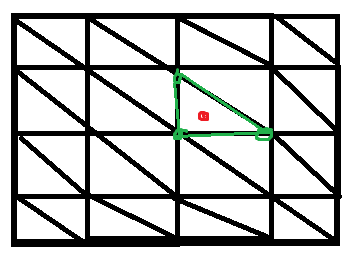
\includegraphics[scale=0.5]{CollisionTerrain.png}
  \end{center}
  \caption{Collision with Terrain}
\end{wrapfigure}

To Calculate the Collision Face, we have taken the three nearest Terrain Heightmap point to our Point mapped on the Heightmap Array. \\
The second step is to calculate the Triangle with the point of the flake. We simply can take 2 random points from the collision Face mentioned before and the one from the position of the Flake. 
Now we can calculate the dot Product of the normal of the triangles and take the “collisionDistanceThereshold” Parameter mentioned in the top of the Particle Class to check if it’s nearly zero..\\

\subsubsection{Collision Response}
We already know if our Flake is colliding with the Ground. The next Step is to calculate the Response of the Flake after the collision with the Terrain. I first show the code: \\
\begin{lstlisting} [language=Python]
outputVector = np.add(-2 * np.dot(self.speed, 
normalizedNormale) * 
normalizedNormale, self.speed)

return outputVector/np.linalg.norm(
outputVector) * np.linalg.norm(self.speed)
\end{lstlisting}
With this code, we solve a Problem I describe in some pictures. 
V is our actual speed, which is the vector we collide with the Terrain. R is the output Vector after the Collision. N is the normal of the collision Face. 

\begin{wrapfigure}{r}{0.5\textwidth}
  \begin{center}
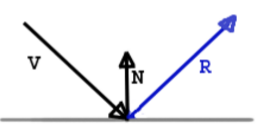
\includegraphics[scale=0.5]{CollisionResponse1Terrain.png}
  \end{center}
  \caption{Collisionresponse 1}
\end{wrapfigure}
\begin{wrapfigure}{r}{0.5\textwidth}
  \begin{center}
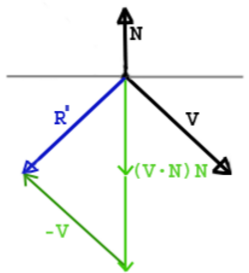
\includegraphics[scale=0.5]{CollisionResponse2Terrain.png}
  \end{center}
  \caption{Collisionresponse 2}
\end{wrapfigure}

 To now get R’ which is the negative of R we need to dot Product V with the normal of the Collision Face N multiplied with N to map V on the Axis of the normal of the Collision Face. After this we have to double this Vector, to get the correct vector length of the new Vector on the normal of the Collision Face. After that we subtract V from this to get the Vector R’. Now we have the negated R, which is our output Vector. Simply negate R’ to get R. \\
This output Vector is the Force which will have impact on the new speed of the Flake. \\
With: 
\begin{lstlisting} [language=Python]
self.speed[0] = collisionForce[0] 
* self.elasticity
self.speed[1] = collisionForce[1] 
* self.elasticity
self.speed[2] = collisionForce[2] 
* self.elasticity
\end{lstlisting}
The new Speed is set to the force calculated before. Of course we have to multiply it with the elasticity of the flake. \\
\\

\section{Conclusion and Outlook}
@Tiras Dinge ausschreiben
- enable Mass is related to size of Particle and force
- extend camera rotation, translation with mouse and keyboard
- multiple terrains, mutiple flakes
- debug mode enabled while running. More Debug Modes like coloring flakes for more speed
- enable friction of Terrain
- better performance to really have an Avalanche

\bibliographystyle{abbrv}
\bibliography{sigproc} 

\end{document}
